\documentclass[tikz,border=7pt]{standalone}
\usepackage{pgfplots}
\pgfplotsset{compat=1.18}
\begin{document}
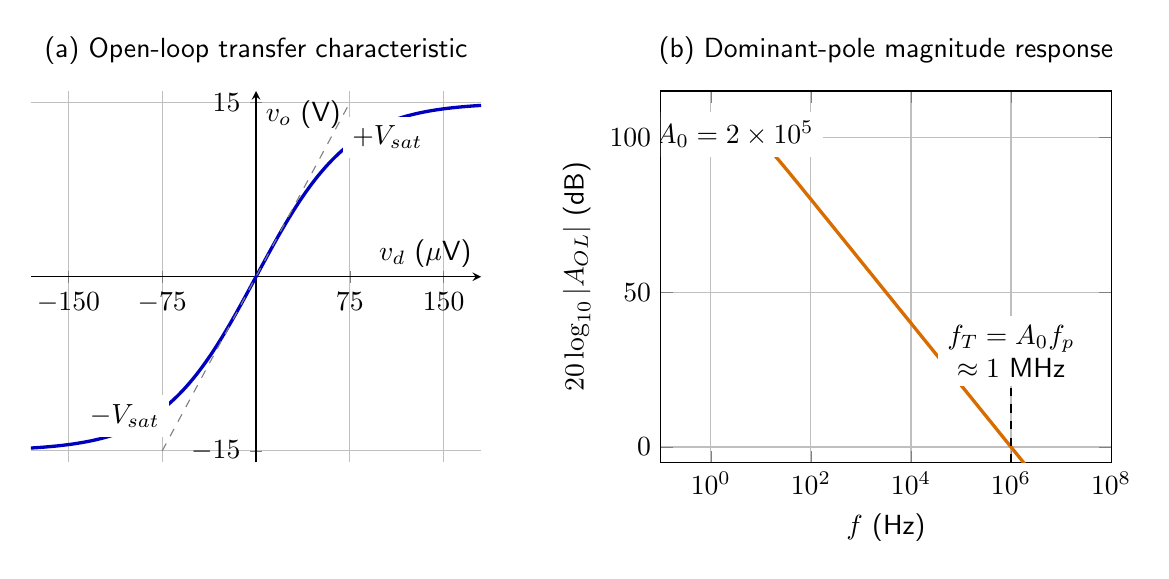
\begin{tikzpicture}[font=\sffamily]
 \begin{axis}[name=a,width=7.3cm,height=6.3cm,axis lines=middle,
 xlabel={$v_d$ ($\mu$V)},ylabel={$v_o$ (V)},xmin=-180,xmax=180,ymin=-16,ymax=16,
 xtick={-150,-75,0,75,150},ytick={-15,0,15},grid=both,
 title={(a) Open-loop transfer characteristic}]
  \addplot[blue!75!black,very thick,domain=-180:180,samples=220]
   {15*tanh(x/75)};
  \addplot[dashed,gray,domain=-75:75] {0.2*x};
  \node[fill=white] at (axis cs:105,12) {$+V_{sat}$};
  \node[fill=white] at (axis cs:-105,-12) {$-V_{sat}$};
 \end{axis}
 \begin{semilogxaxis}[at={(8cm,0)},anchor=south west,width=7.3cm,height=6.3cm,
 xlabel={$f$ (Hz)},ylabel={$20\log_{10}|A_{OL}|$ (dB)},xmin=.1,xmax=1e8,
 ymin=-5,ymax=115,grid=both,title={(b) Dominant-pole magnitude response},
 xtick={1,1e2,1e4,1e6,1e8}]
  \addplot[orange!85!black,very thick,domain=.1:1e8,samples=250]
  {20*log10(2e5/sqrt(1+(x/5)^2))};
  \draw[dashed] (axis cs:1e6,-5) -- (axis cs:1e6,20);
  \node[fill=white,align=center] at (axis cs:1e6,31) {$f_T=A_0f_p$\\$\approx1$ MHz};
  \node[fill=white] at (axis cs:3,101) {$A_0=2\times10^5$};
 \end{semilogxaxis}
\end{tikzpicture}
\end{document}
